\documentclass[../verslag.tex]{subfiles}
\graphicspath{{\subfix{../images/}}}
\begin{document}

De gemiddelde sluis bestaat uit drie delen met twee schuiven die deze delen scheiden. Wanneer het hoogte verschil van het water heel groot is zijn er vaak meerdere delen en schuiven. In dit scenario gaan we er van uit dat deze sluis drie delen en twee schuiven heeft. Ook heeft deze sluis aan elke schuif een groen licht en een rood licht. Deze stoplichten zijn aan beide kanten van de schuiven zichtbaar.

Er komt een boot aan aan de linker kant van de sluis. Het waterniveau aan de rechter kant is hoger dan het waterniveau aan de linker kant van de sluis. Er is een stoplicht met een rood brandend licht die aan geeft dat doorvaart verboden is.

\begin{figure}[H]
	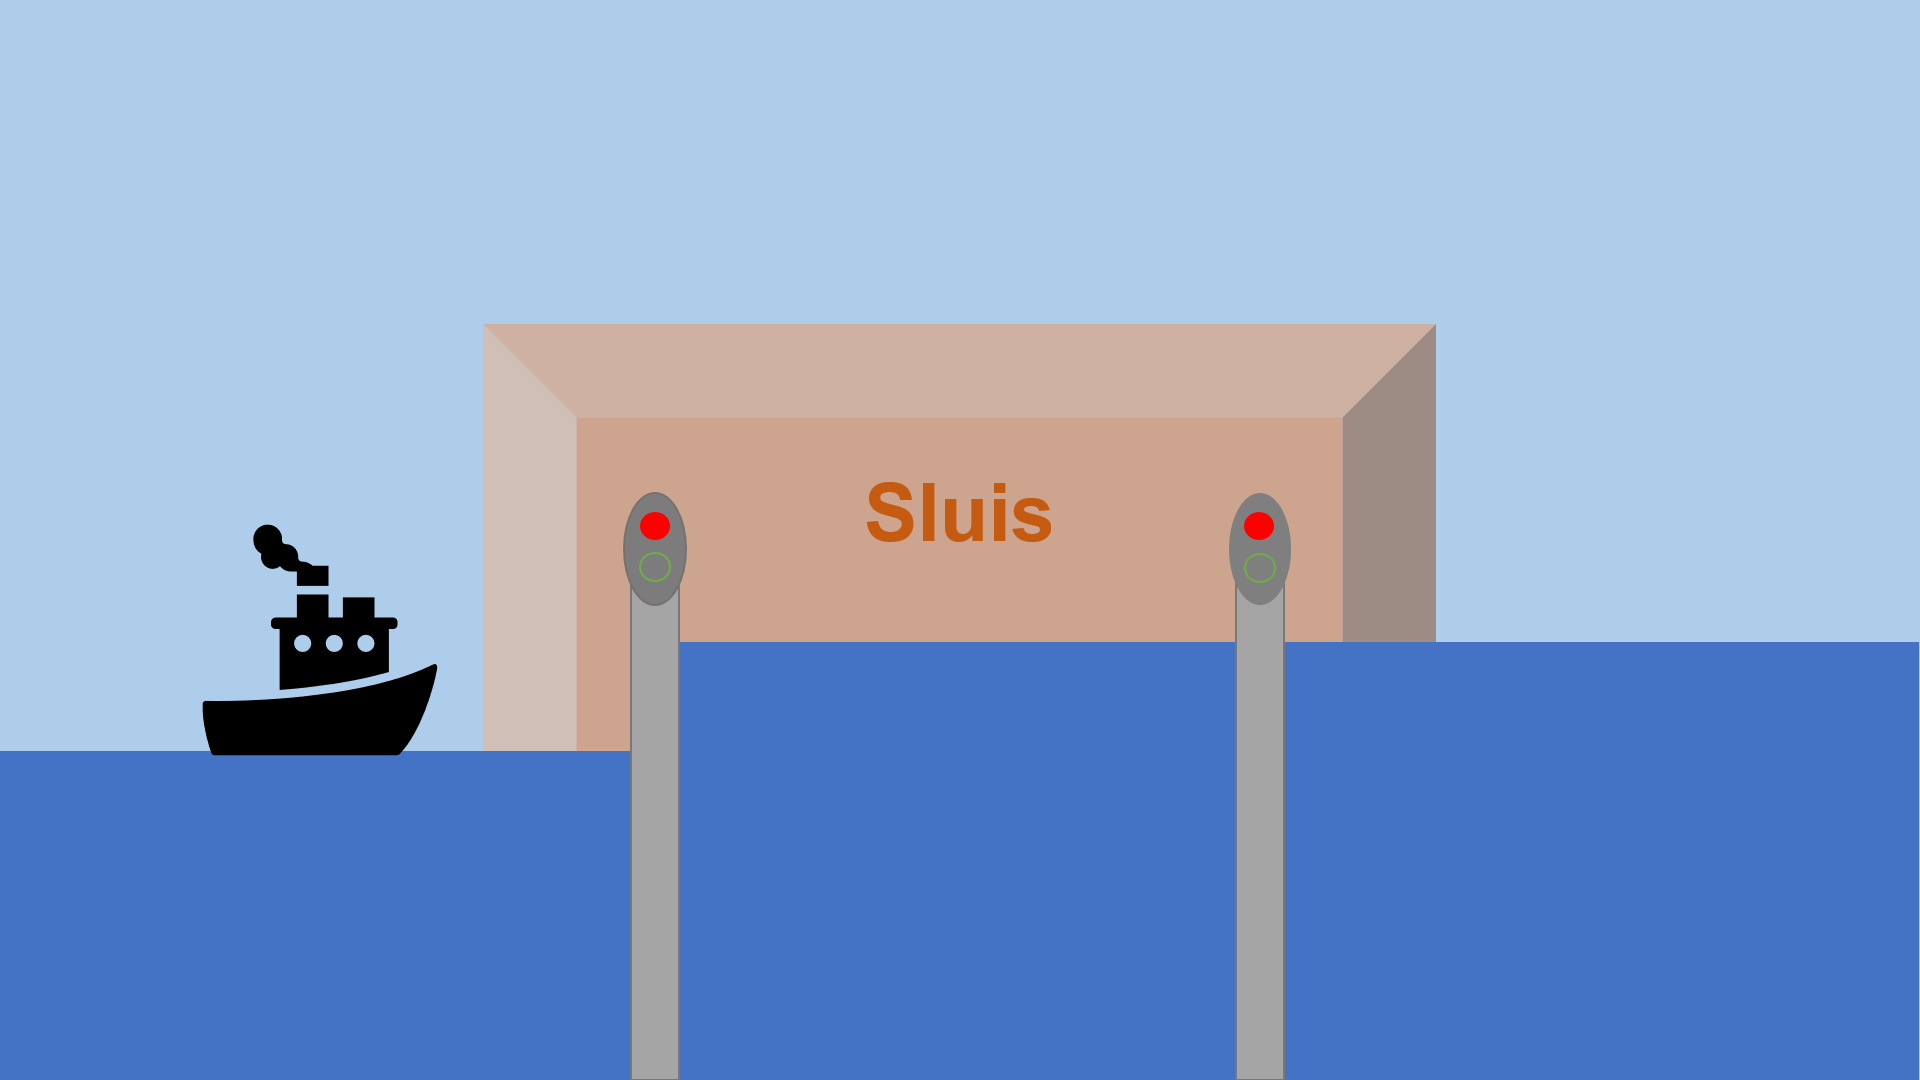
\includegraphics[width=8cm]{Sluis_Operatie1.png}
	\caption{
		Er komt een boot aan bij de sluis, die naar de andere kant moet.
	}
	\label{sluis_op1}
\end{figure}

Om de boot door de sluis heen te krijgen moet eerst het waterniveau in de sluis zakken naar het niveau aan de linker kant. De linker schuif gaat omhoog, hierdoor gaat het water in de sluis weg naar de linkerkant.

\begin{figure}[H]
	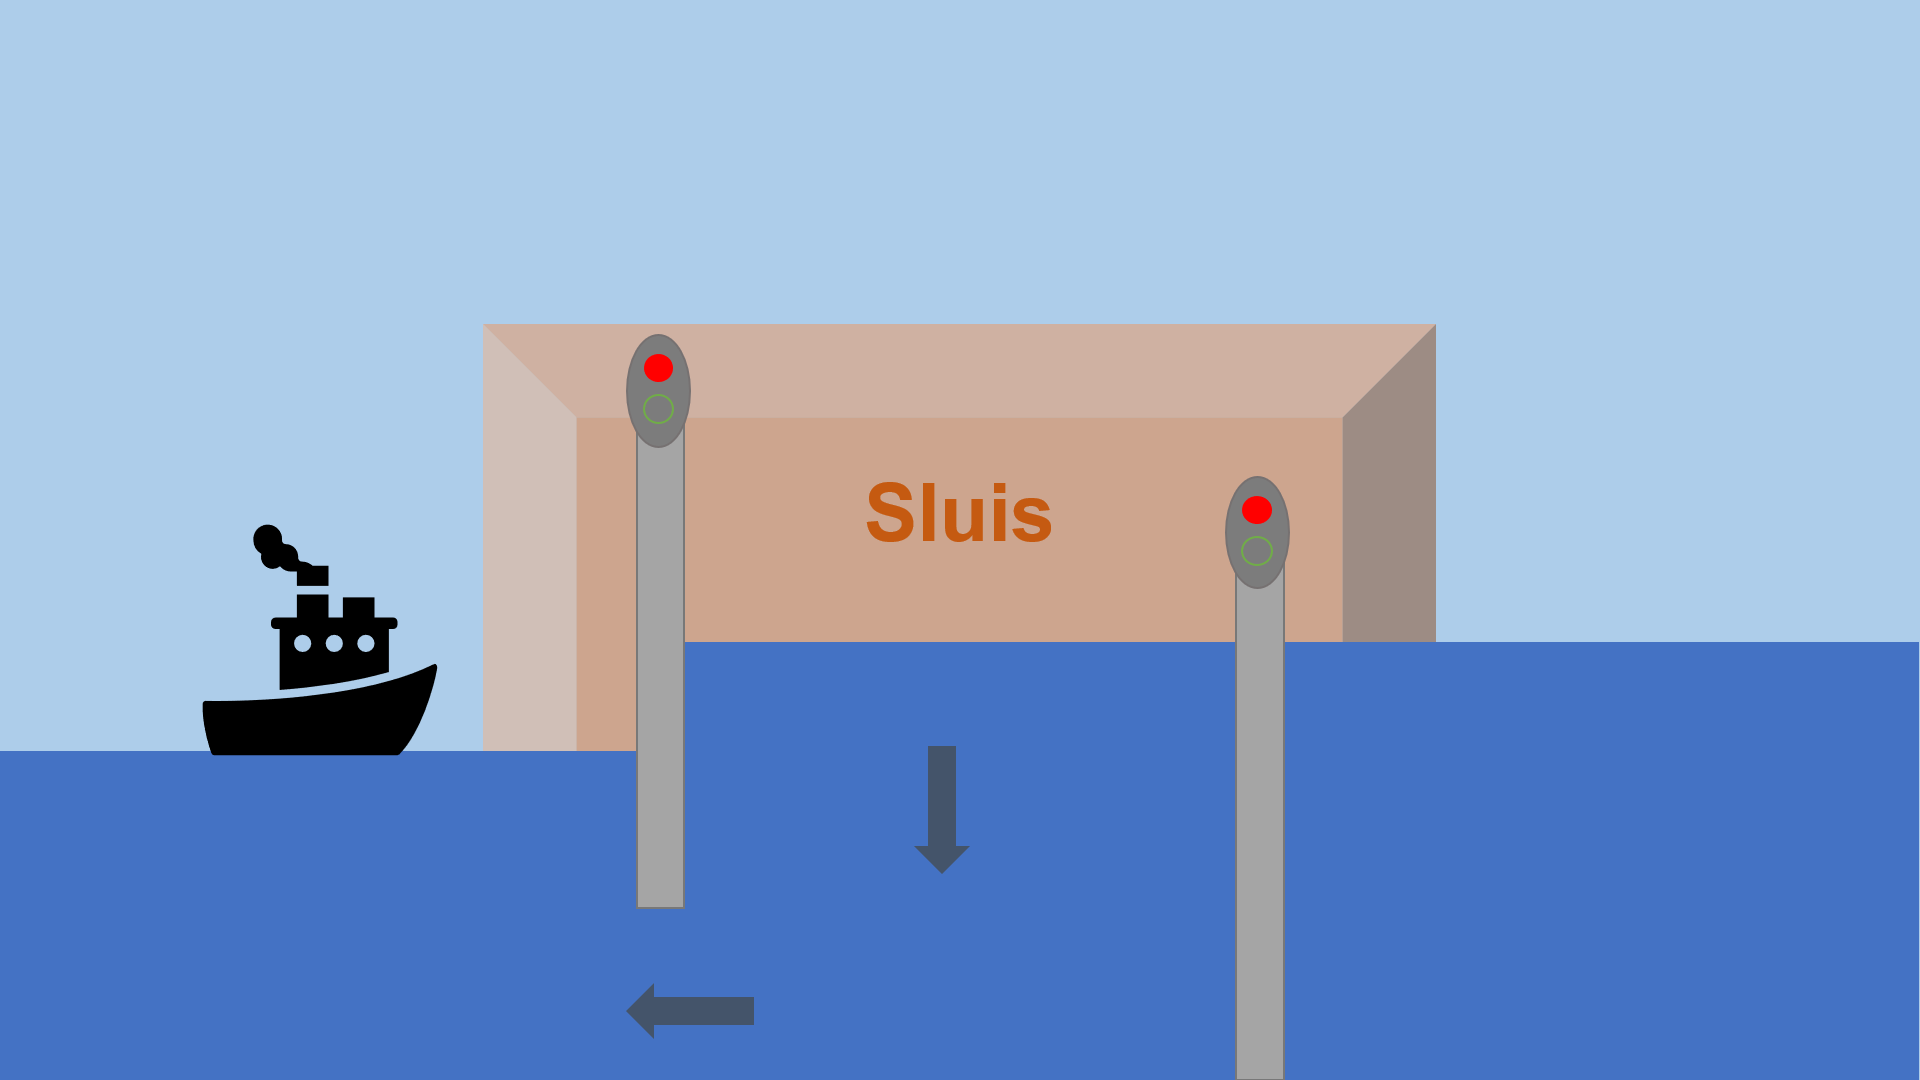
\includegraphics[width=8cm]{Sluis_Operatie2.png}
	\caption{
		De linker schuif gaat omhoog om het waternivea in de sluis gelijk te krijgen.
	}
	\label{sluis_op2}
\end{figure}

Wanneer het waterniveau aan de linker kant en in de sluis gelijk is zakt de schuif naar beneden en gaan de deuren van de schuif open. Het groene licht brand nu om aan te geven dat doorvaart toegestaan is.

\begin{figure}[H]
	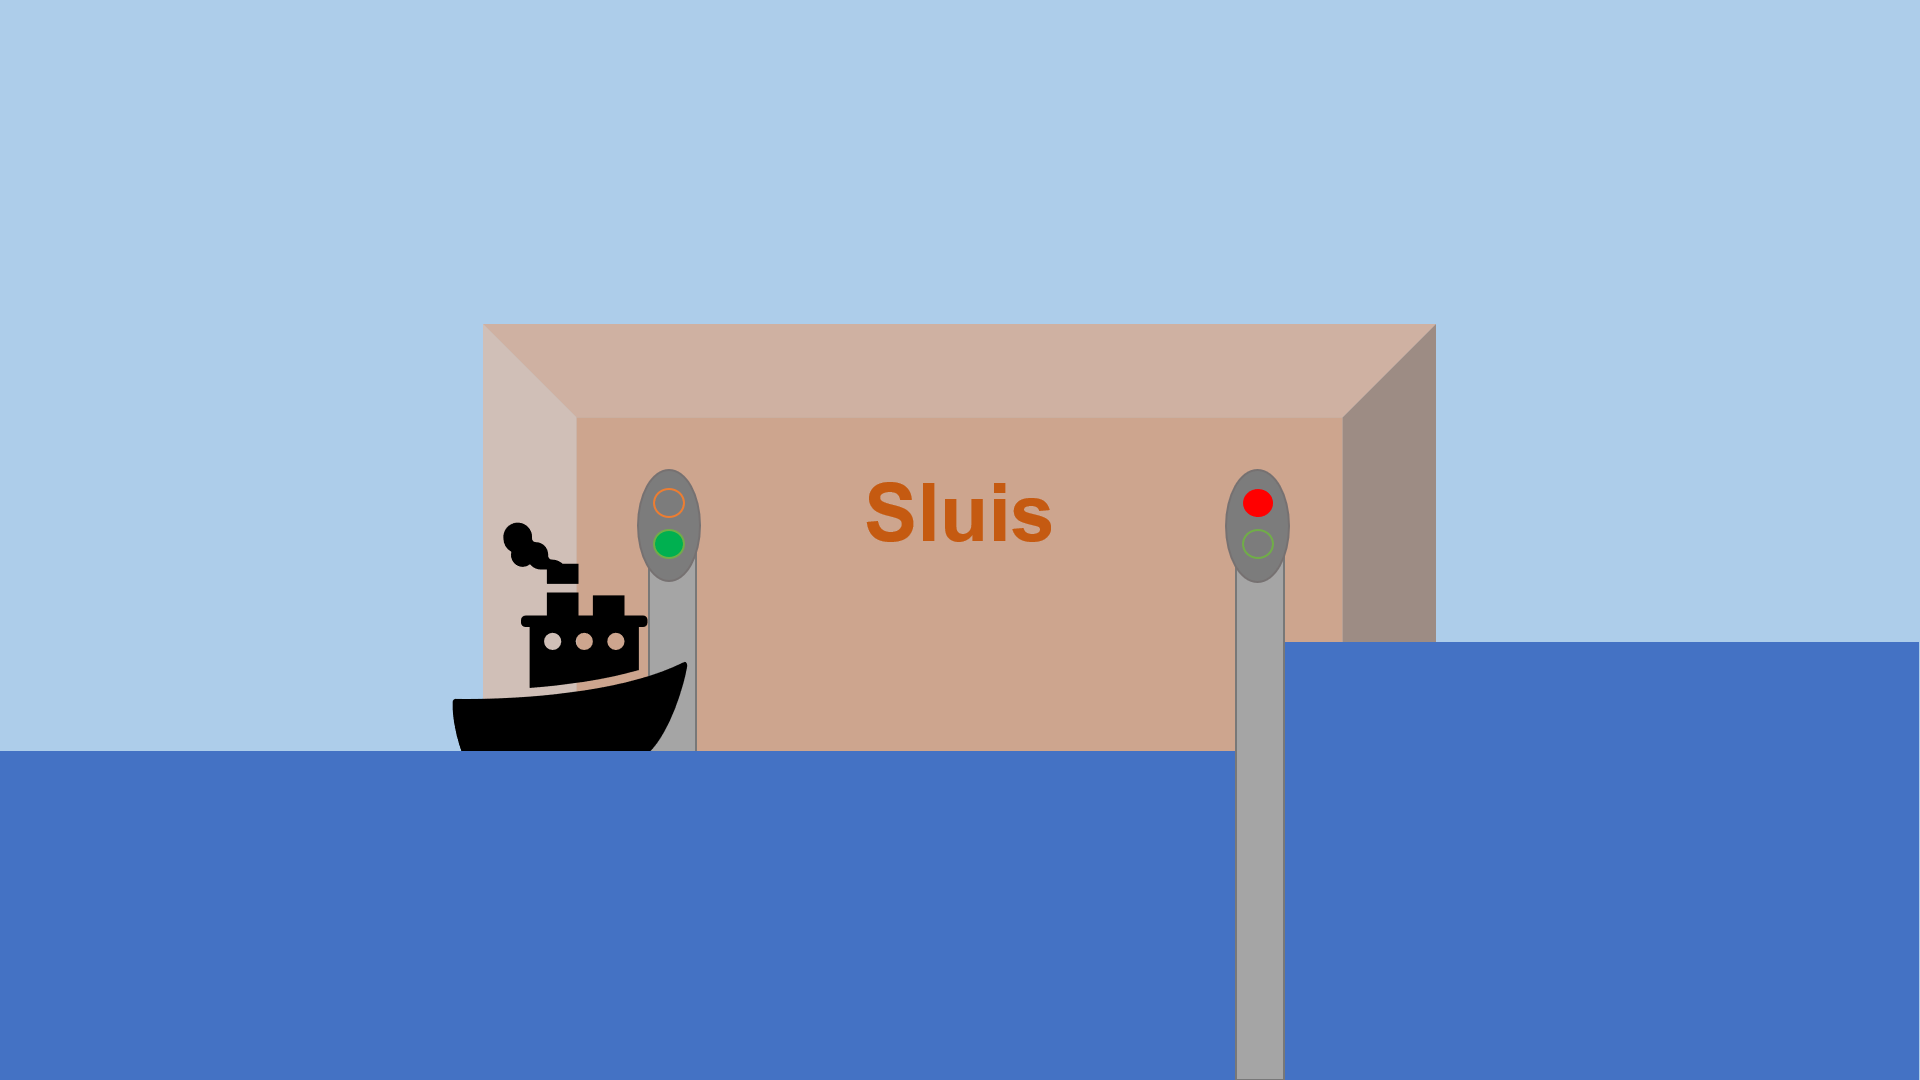
\includegraphics[width=8cm]{Sluis_Operatie3.png}
	\caption{
		Het linker groene licht brand en de boot vaart de sluis in.
	}
	\label{sluis_op3}
\end{figure}

De deuren van de linker schuif gaan dicht als de boot in de sluis is. Het licht van de linker schuif gaat weer naar rood.

\begin{figure}[H]
	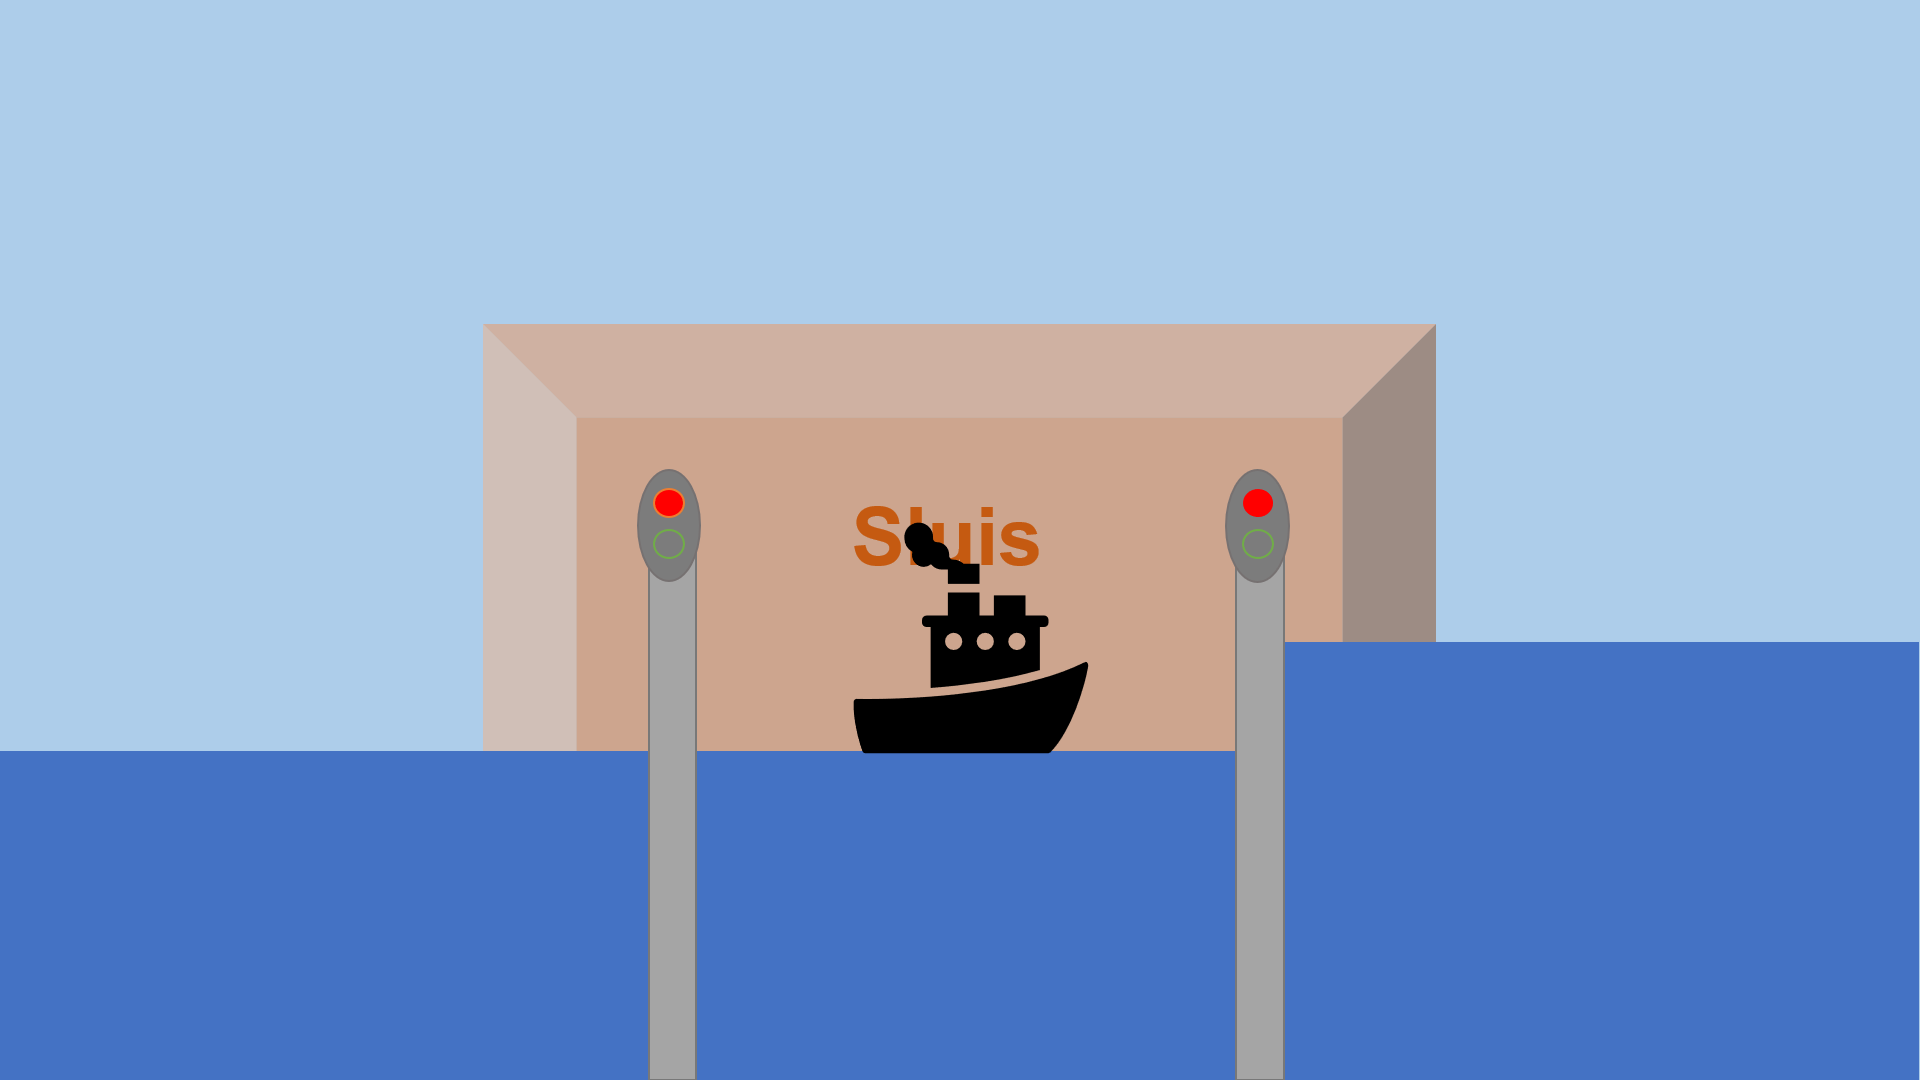
\includegraphics[width=8cm]{Sluis_Operatie4.png}
	\caption{
		De boot wacht in de sluis.
	}
	\label{sluis_op4}
\end{figure}

Het waterniveau moet nu gelijk worden met het niveau aan de linker kant. De rechter schuif gaat nu omhoog. Het waterniveau in de sluis wordt nu gelijk met de rechterkant.

\begin{figure}[H]
	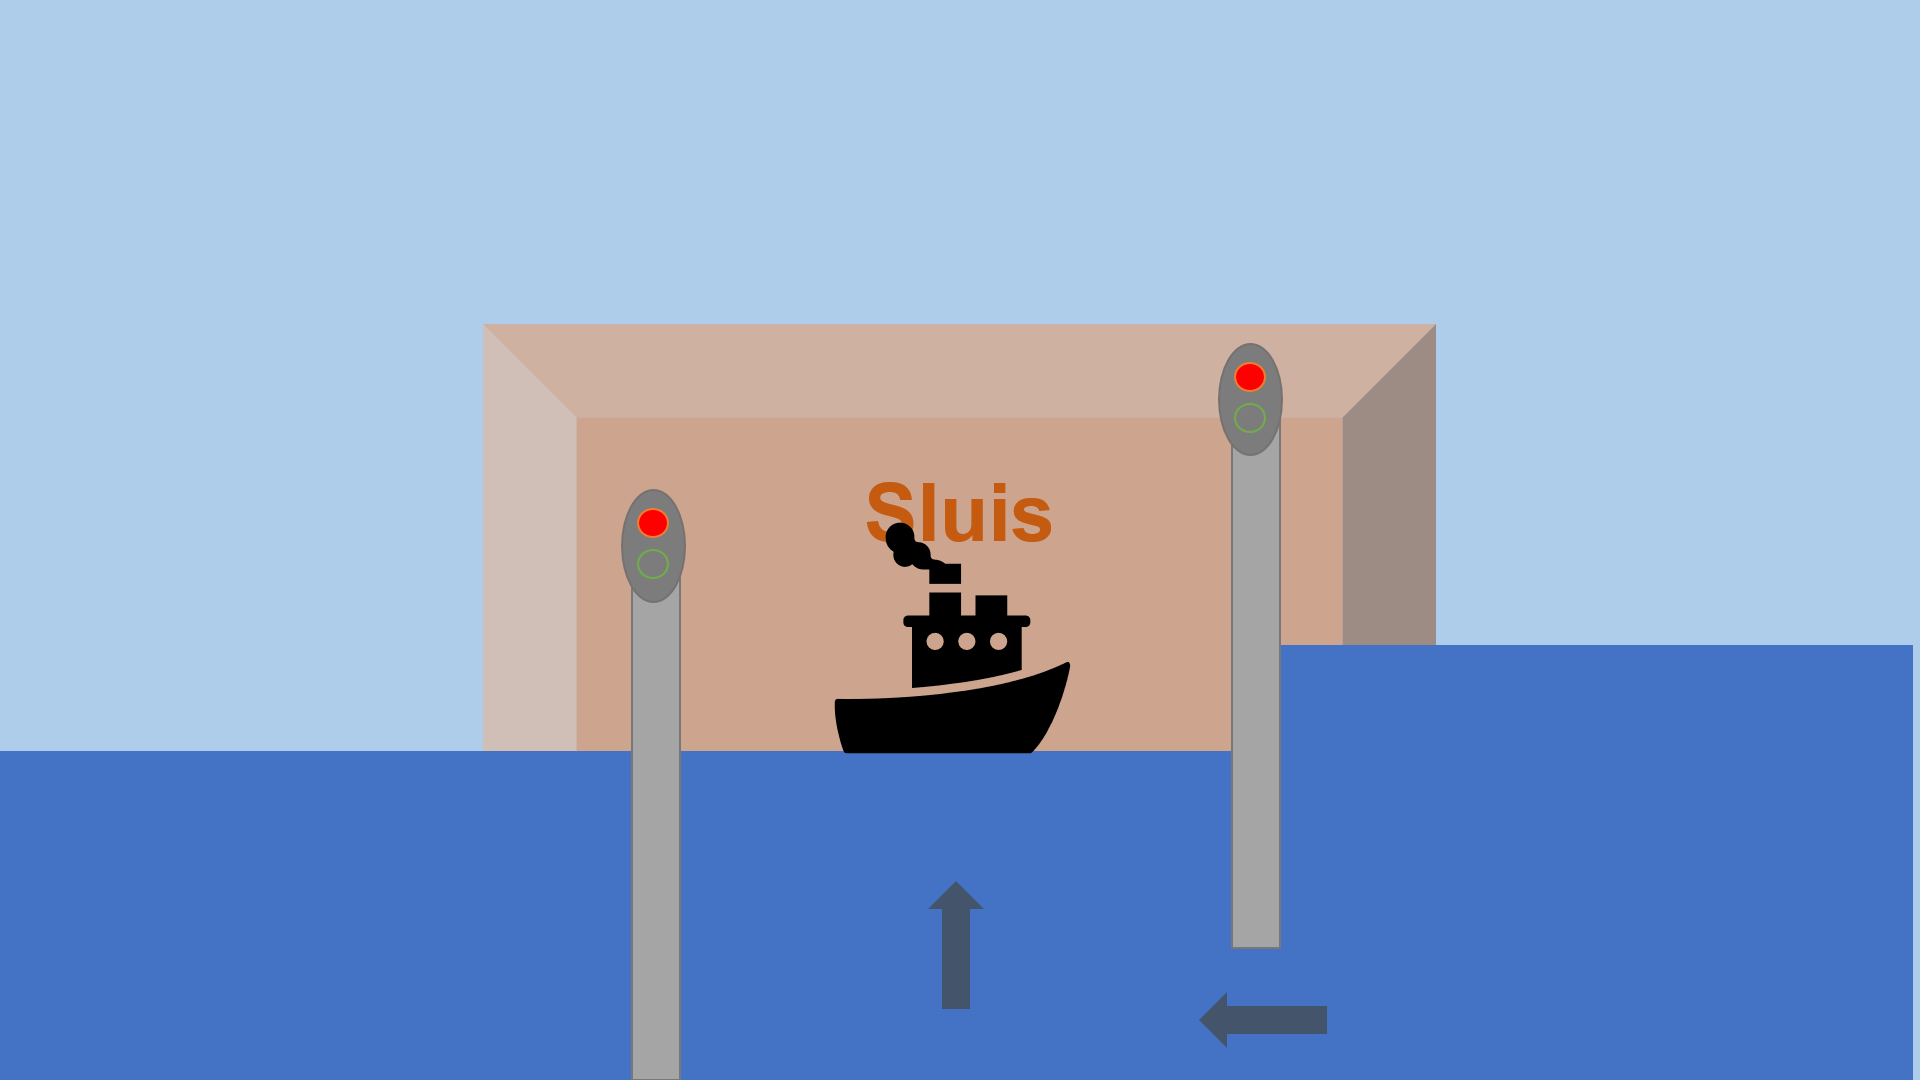
\includegraphics[width=8cm]{Sluis_Operatie5.png}
	\caption{
		De rechter schuif gaat omhoog om het waternivea in de sluis gelijk te krijgen.
	}
	\label{sluis_op5}
\end{figure}

Wanneer het waterniveau aan de rechterkant en in de sluis gelijk is zakt de schuif weer naar beneden.

\begin{figure}[H]
	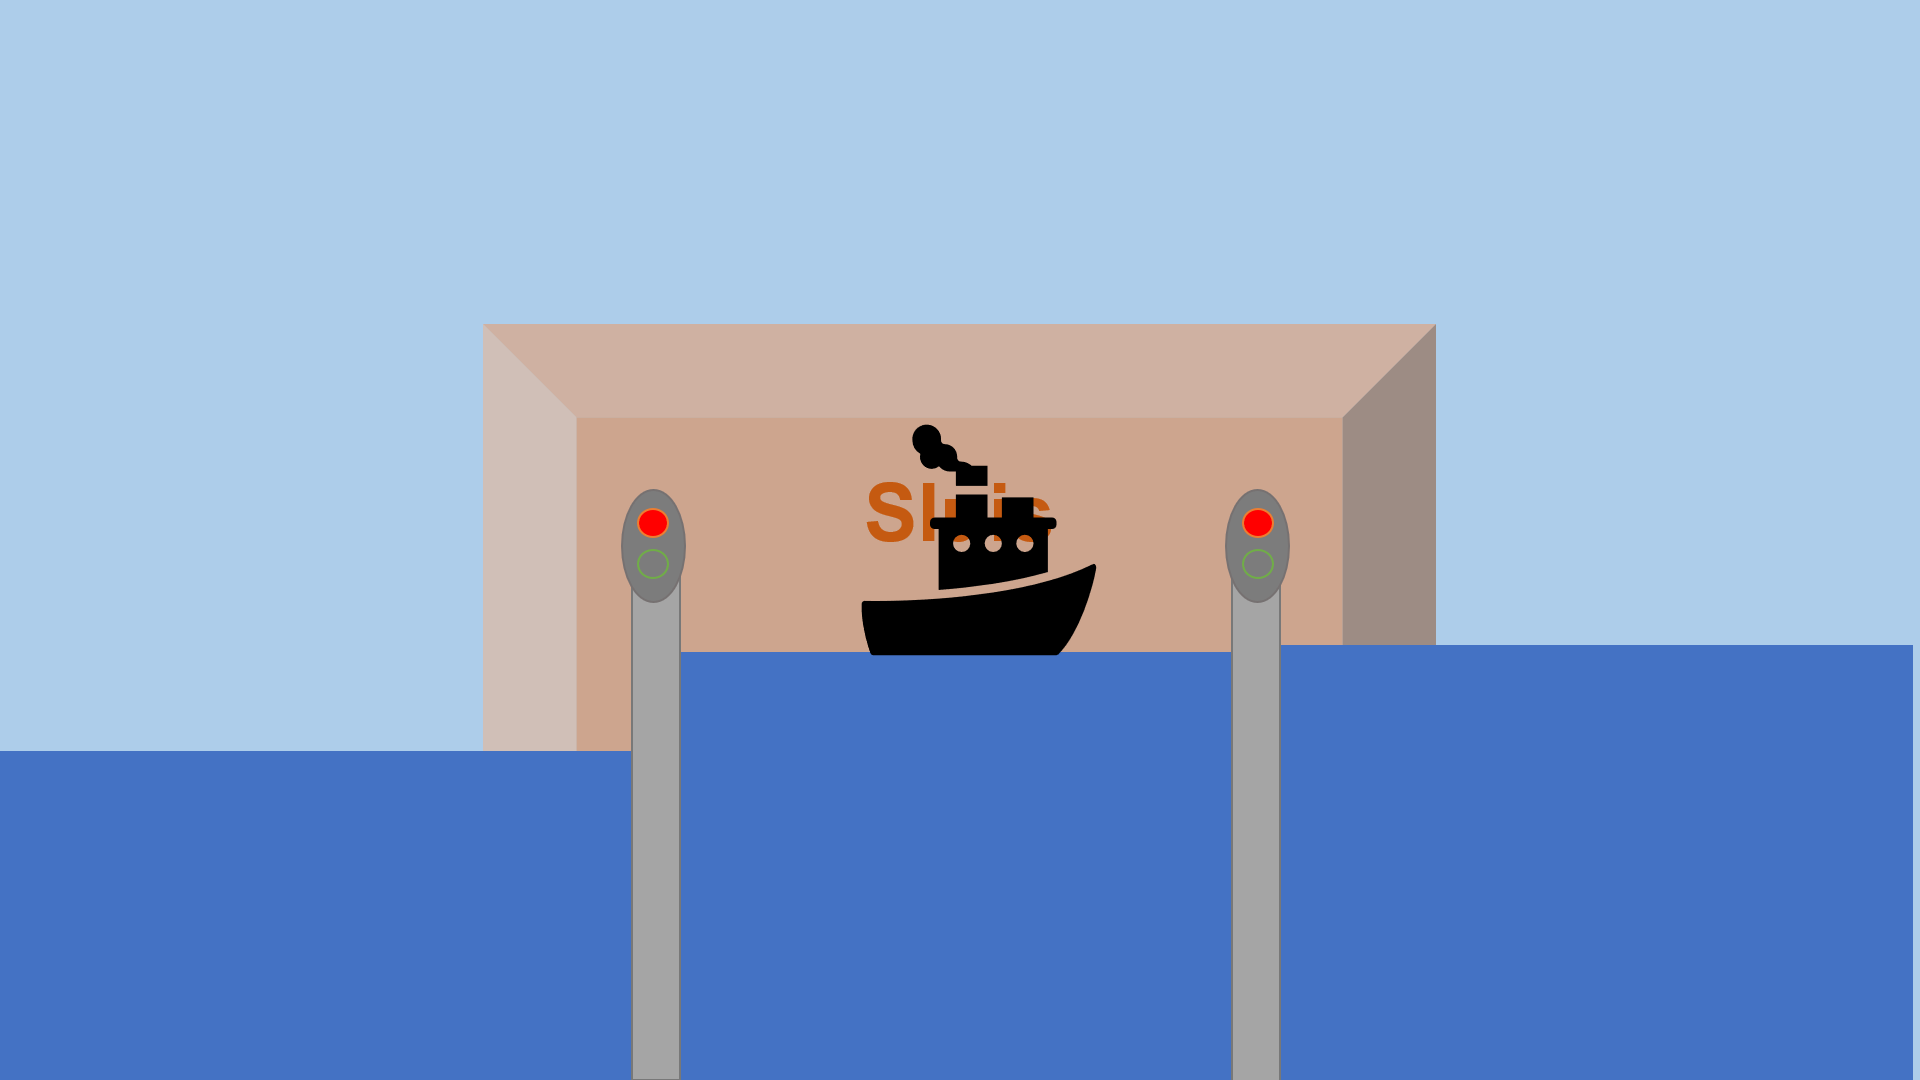
\includegraphics[width=8cm]{Sluis_Operatie6.png}
	\caption{
		Het waterniveau in de sluis is nu gelijk met de rechterkant.
	}
	\label{sluis_op6}
\end{figure}

De deuren van van de rechter schuif gaan nu open en het groene licht gaat branden. De boot vaart naar de rechterkant uit de sluis.

\begin{figure}[H]
	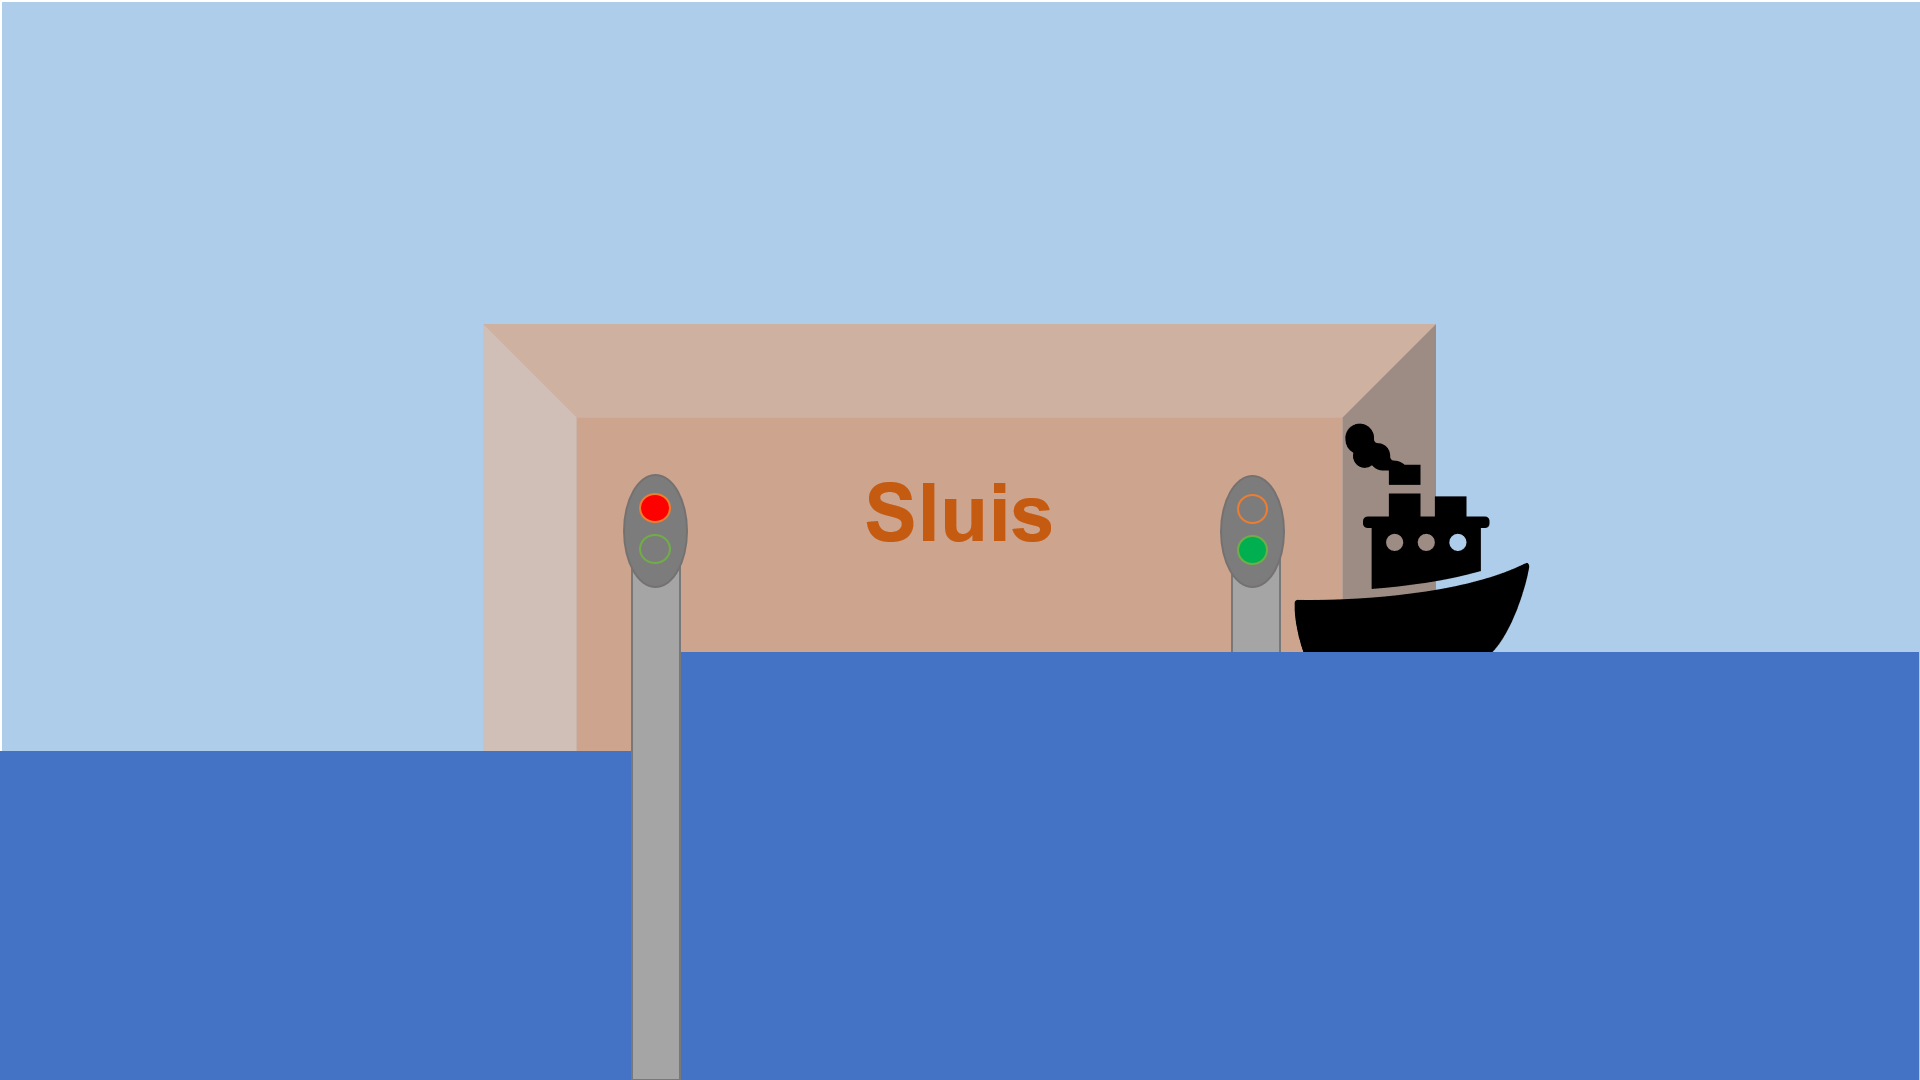
\includegraphics[width=8cm]{Sluis_Operatie7.png}
	\caption{
		Het waterniveau in de sluis is nu gelijk met de rechterkant.
	}
	\label{sluis_op7}
\end{figure}

\end{document}
